\subsubsection{Iteration 3: Test Flight in a Realistic Environment}

\paragraph{Redesign}

Findings from the previous iteration indicated that users experienced difficulty in maintaining spatial orientation during first-person flight. The skybox environment did not provide sufficient visual cues for direction perception.

To address this limitation, a realistic urban environment was introduced. Based on publicly available datasets \parencite{TallinnCityModel2012, EstonianLandBoard2020}, a 3D model of Tallinn was imported into Unity to construct the simulation environment (see \cref{fig:tallinn}).

Within this environment, a goal-oriented task was designed in which the player navigates from Viru Gate to Tallinn Town Hall. Directional signs and collectible elements (e.g., coins) were implemented to provide guidance and reinforce goal-directed navigation.

\paragraph{Enactment}

The imported city model and terrain are shown in \cref{fig:tallinn}. To ensure real-time performance in XR, occlusion culling was applied to reduce rendering load by excluding non-visible geometry.

\begin{figure}[H]
    \caption{The Tallinn Old Town model (top) and terrain (bottom) imported into Unity}\label{fig:tallinn}
    \centering
    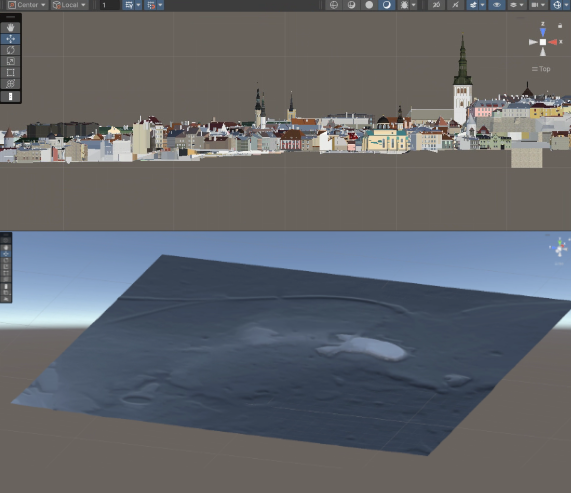
\includegraphics[width=0.6\linewidth]{img/Tallinn.png}
\end{figure}

After refinement of the skybox and building materials, the final environment is presented in \cref{fig:realistic}, including the navigation route, player view, collectible elements, and mesh-based collision boundaries.

\begin{figure}[H]
    \caption{Navigation route in the green collider (top), player view (bottom-left), and coin collection with mesh collider (bottom-right)}\label{fig:realistic}
    \centering
    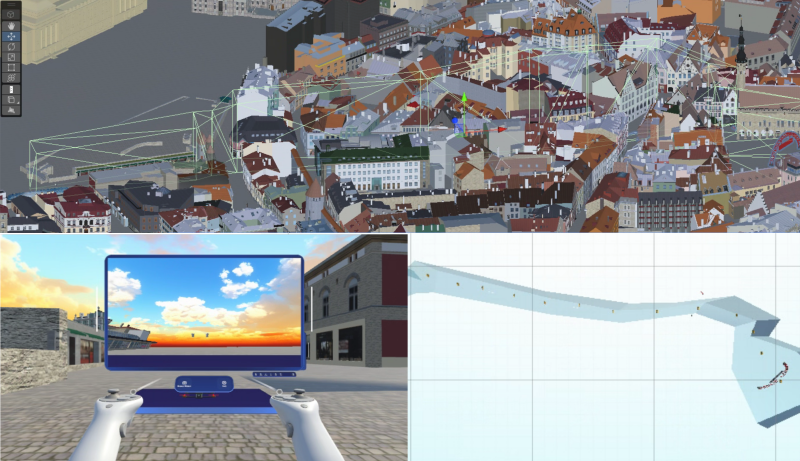
\includegraphics[width=0.6\linewidth]{img/real.png}
\end{figure}

\paragraph{Analysis}

The introduction of a realistic environment significantly enhanced user engagement and perceived immersion. Play tests shows that the enriched visual context improved their ability to orient themselves during flight.

Some participants suggested enabling free exploration of the environment, aligning with the active experimentation stage of experiential learning.

At the same time, the increased visual complexity led to performance challenges in XR rendering. Several testers proposed the use of simplified or white-box environments to lower down the performance issue.